\documentclass[11pt,a4paper]{article}
\usepackage[utf8]{inputenc}\usepackage[T1]{fontenc}\usepackage{lmodern}\usepackage{microtype}
\usepackage[margin=1in]{geometry}
\usepackage{amsmath}\usepackage{booktabs}\usepackage{graphicx}\usepackage{xcolor}\usepackage{enumitem}\usepackage{array}
\usepackage[font=small,labelfont=bf,skip=3pt]{caption}
\usepackage{tikz}\usetikzlibrary{arrows.meta}
\usepackage[authoryear,round]{natbib}\bibpunct{(}{)}{;}{a}{,}{,}
\usepackage[colorlinks=true,linkcolor=blue!50!black,citecolor=blue!50!black,urlcolor=blue!50!black]{hyperref}
\usepackage[compact]{titlesec}\titlespacing*{\section}{0pt}{8pt}{3pt}\titlespacing*{\subsection}{0pt}{5pt}{2pt}
\setlength{\parskip}{0pt}\setlength{\parindent}{1.2em}\setlist{nosep,leftmargin=1.4em}
\setlength{\textfloatsep}{7pt plus 2pt minus 2pt}\setlength{\floatsep}{5pt plus 2pt minus 2pt}\setlength{\intextsep}{5pt plus 2pt minus 2pt}
% AUTO-GENERATED by analysis/50_make_report_inputs.py - do not edit by hand
\newcommand{\nEventsScope}{512{,}821}
\newcommand{\nStudents}{10{,}044}
\newcommand{\nExits}{9{,}426}
\newcommand{\nSessions}{83{,}224}
\newcommand{\sessionExitRate}{11.3\%}
\newcommand{\dsSessions}{83{,}224}
\newcommand{\dsStudents}{10{,}044}
\newcommand{\nEventsRaw}{641{,}490}
\newcommand{\nSessionsMulti}{6{,}348}
\newcommand{\qOneFailedRetries}{52{,}190}
\newcommand{\qOneRoute}{44{,}190}
\newcommand{\qOneStudents}{5{,}544}
\newcommand{\qOneLesson}{39{,}467}
\newcommand{\qOneSkip}{4{,}723}
\newcommand{\qOneSkipShare}{10.7\%}
\newcommand{\qOneSuccSkip}{34.7\%}
\newcommand{\qOneSuccSkipCI}{33.4 to 36.1}
\newcommand{\qOneEvSkip}{4{,}723}
\newcommand{\qOneSuccGlance}{35.7\%}
\newcommand{\qOneSuccGlanceCI}{34.1 to 37.6}
\newcommand{\qOneEvGlance}{8{,}004}
\newcommand{\qOneSuccRead}{50.1\%}
\newcommand{\qOneSuccReadCI}{49.1 to 51.2}
\newcommand{\qOneEvRead}{23{,}799}
\newcommand{\qOneSuccLong}{51.1\%}
\newcommand{\qOneSuccLongCI}{49.7 to 52.5}
\newcommand{\qOneEvLong}{7{,}664}
\newcommand{\qOneMedRead}{22}
\newcommand{\qOneMedGlance}{6}
\newcommand{\qOneEffRaw}{12.7}
\newcommand{\qOneEffRawCI}{11.3 to 14.2}
\newcommand{\qOneEffSame}{13.0}
\newcommand{\qOneEffSameCI}{10.7 to 15.4}
\newcommand{\qOneEffFE}{5.9}
\newcommand{\qOneEffFECI}{4.3 to 7.5}
\newcommand{\qOneEffLogit}{7.0}
\newcommand{\qOneEffLogitCI}{5.4 to 8.6}
\newcommand{\qOneEffIPW}{8.3}
\newcommand{\qOneEffIPWCI}{6.2 to 10.4}
\newcommand{\qOneOR}{1.34}
\newcommand{\qOneORCI}{1.25 to 1.44}
\newcommand{\qOnePlacebo}{0.2}
\newcommand{\qOnePlaceboCI}{$-$0.6 to 1.0}
\newcommand{\qOnePlaceboRaw}{22.7}
\newcommand{\qOneFEBefore}{5.1}
\newcommand{\qOneFEBeforeCI}{2.9 to 7.3}
\newcommand{\qOneFEAfter}{7.0}
\newcommand{\qOneFEAfterCI}{4.3 to 9.6}
\newcommand{\qOneFENoLong}{6.0}
\newcommand{\qOneFENoLongCI}{4.4 to 7.6}
\newcommand{\qOneFEQFour}{4.9}
\newcommand{\qOneFEQFourCI}{2.9 to 6.9}
\newcommand{\qOneRR}{1.17}
\newcommand{\qOneEvalue}{1.62}
\newcommand{\qOneEvalueCI}{1.52}
\newcommand{\qOneSMDfail}{1.09}
\newcommand{\qOneSMDacc}{0.65}
\newcommand{\qOneSkipEarlierFail}{5.2}
\newcommand{\qOneLessonEarlierFail}{2.5}
\newcommand{\qOneDoseFEGlance}{2.8}
\newcommand{\qOneDoseFEGlanceCI}{0.8 to 4.8}
\newcommand{\qOneDoseFERead}{7.4}
\newcommand{\qOneDoseFEReadCI}{5.7 to 9.1}
\newcommand{\qOneDoseFELong}{6.1}
\newcommand{\qOneDoseFELongCI}{4.1 to 8.2}
\newcommand{\qTwoRateFR}{13.1\%}
\newcommand{\qTwoRateFRCI}{12.0 to 14.2}
\newcommand{\qTwoRateOther}{0.94\%}
\newcommand{\qTwoRatio}{13.9}
\newcommand{\qTwoRatioCI}{12.9 to 14.9}
\newcommand{\qTwoShareFR}{57\%}
\newcommand{\qTwoToLesson}{78.8\%}
\newcommand{\qTwoToCheckout}{7.6\%}
\newcommand{\qTwoToQuit}{13.1\%}
\newcommand{\qTwoToNext}{0.5\%}
\newcommand{\qTwoQuitAfterLesson}{0.003\%}
\newcommand{\qTwoStudentRateFR}{27\%}
\newcommand{\qTwoStudentRateFRCI}{26 to 28}
\newcommand{\qTwoNStepsFR}{40{,}787}
\newcommand{\qTwoCommitNoLesson}{10\%}
\newcommand{\qTwoCommitLesson}{0.0\%}
\newcommand{\qTwoRateBefore}{9.2\%}
\newcommand{\qTwoRatioBefore}{13.6}
\newcommand{\qTwoRateAfter}{16.7\%}
\newcommand{\qTwoRatioAfter}{14.7}
\newcommand{\qTwoICCStudent}{0.285}
\newcommand{\qTwoICCStudentCI}{0.254 to 0.316}
\newcommand{\qTwoICCTopic}{0.012}
\newcommand{\qTwoICCTopicCI}{0.009 to 0.016}
\newcommand{\qTwoICCConcept}{0.027}
\newcommand{\qTwoICCConceptCI}{0.020 to 0.034}
\newcommand{\hzAUCA}{0.769}
\newcommand{\hzRA}{0.161}
\newcommand{\hzAUCB}{0.804}
\newcommand{\hzRB}{0.173}
\newcommand{\hzAUCC}{0.803}
\newcommand{\hzRC}{0.174}
\newcommand{\hzAUCD}{0.824}
\newcommand{\hzRD}{0.185}
\newcommand{\hzAUCE}{0.853}
\newcommand{\hzRE}{0.215}
\newcommand{\hzMargLatA}{6.9\%}
\newcommand{\hzMargLatB}{9.4\%}
\newcommand{\hzMargLatC}{13.0\%}
\newcommand{\hzMargLatD}{14.0\%}
\newcommand{\hzMargLatE}{12.9\%}
\newcommand{\hzMargLatF}{14.7\%}
\newcommand{\hzMargFailZero}{13.8\%}
\newcommand{\hzMargFailOne}{10.4\%}
\newcommand{\hzMargFailTwo}{8.6\%}
\newcommand{\hzMargFailThree}{6.6\%}
\newcommand{\hzMargPosOne}{17.2\%}
\newcommand{\hzMargPosTwo}{13.7\%}
\newcommand{\hzMargPosThree}{11.4\%}
\newcommand{\hzMargPosFour}{9.7\%}
\newcommand{\hzFEFailOne}{1.65}
\newcommand{\hzFEFailOneCI}{1.47 to 1.85}
\newcommand{\hzPoolFailOne}{0.72}
\newcommand{\hzFEFailTwo}{1.98}
\newcommand{\hzFEFailTwoCI}{1.55 to 2.53}
\newcommand{\hzPoolFailTwo}{0.58}
\newcommand{\hzFEPosFour}{0.42}
\newcommand{\hzFEPosFourCI}{0.37 to 0.48}
\newcommand{\hzPoolPosFour}{0.51}
\newcommand{\hzFEAfter}{4.22}
\newcommand{\hzFEAfterCI}{3.69 to 4.82}
\newcommand{\hzPoolAfter}{1.70}
\newcommand{\hzFEstudents}{1{,}734}
\newcommand{\cpDate}{3 May}
\newcommand{\cpLo}{26 April}
\newcommand{\cpHi}{9 May}
\newcommand{\cpBefore}{9.2\%}
\newcommand{\cpAfter}{16.7\%}
\newcommand{\cpLR}{511}
\newcommand{\cpPairN}{372}
\newcommand{\cpPairDiff}{11.6}
\newcommand{\cpPairCI}{9.5 to 14.0}
\newcommand{\cpOtherBefore}{0.85\%}
\newcommand{\cpOtherAfter}{1.92\%}
\newcommand{\qThreeAfterExit}{34.7\%}
\newcommand{\qThreeAfterComplete}{7.9\%}
\newcommand{\qThreeRatio}{4.4}
\newcommand{\qThreeRatioCI}{4.0 to 4.7}
\newcommand{\qThreeDiff}{26.8}
\newcommand{\qThreeDiffCI}{24.6 to 28.9}
\newcommand{\qThreePairs}{73{,}180}
\newcommand{\qThreeAfterQuits}{5{,}876}
\newcommand{\qThreeSame}{38.2\%}
\newcommand{\qThreeWeek}{2.6}
\newcommand{\qThreeRaw}{26.8}
\newcommand{\qThreeRawCI}{24.6 to 29.0}
\newcommand{\qThreeLoo}{11.1}
\newcommand{\qThreeLooCI}{9.4 to 12.8}
\newcommand{\qThreeWithin}{4.3}
\newcommand{\qThreeWithinCI}{2.3 to 6.3}
\newcommand{\qThreeSB}{0.72}
\newcommand{\qThreeSplitN}{1{,}751}
\newcommand{\qThreeNever}{41\%}
\newcommand{\qThreeTop}{54\%}
\newcommand{\qThreeGeFive}{3{,}357}
\newcommand{\qThreeCensored}{12\%}
\newcommand{\qThreeRetFRH}{37.6\%}
\newcommand{\qThreeRetFRHCI}{34.8 to 40.5}
\newcommand{\qThreeRetFRD}{43.6\%}
\newcommand{\qThreeRetFRDCI}{40.4 to 46.6}
\newcommand{\qThreeRetFRW}{56.5\%}
\newcommand{\qThreeRetFRWCI}{53.3 to 59.5}
\newcommand{\qThreeRetFRM}{65.8\%}
\newcommand{\qThreeRetFRMCI}{63.2 to 68.2}
\newcommand{\qThreeMedFR}{11~min}
\newcommand{\qThreeSameQuizFR}{0.1\%}
\newcommand{\qThreeNQuitFR}{5{,}328}
\newcommand{\qThreeRetOthH}{23.4\%}
\newcommand{\qThreeRetOthHCI}{21.3 to 25.3}
\newcommand{\qThreeRetOthD}{28.7\%}
\newcommand{\qThreeRetOthDCI}{26.3 to 30.6}
\newcommand{\qThreeRetOthW}{42.0\%}
\newcommand{\qThreeRetOthWCI}{39.2 to 44.4}
\newcommand{\qThreeRetOthM}{52.1\%}
\newcommand{\qThreeRetOthMCI}{49.5 to 54.5}
\newcommand{\qThreeMedOth}{23~h}
\newcommand{\qThreeSameQuizOth}{0.2\%}
\newcommand{\qThreeNQuitOth}{4{,}098}
\newcommand{\qThreeRetDoneH}{47.7\%}
\newcommand{\qThreeRetDoneHCI}{45.7 to 50.0}
\newcommand{\qThreeRetDoneD}{63.6\%}
\newcommand{\qThreeRetDoneDCI}{62.5 to 65.0}
\newcommand{\qThreeRetDoneW}{85.3\%}
\newcommand{\qThreeRetDoneWCI}{84.5 to 85.9}
\newcommand{\qThreeRetDoneM}{90.4\%}
\newcommand{\qThreeRetDoneMCI}{89.9 to 90.9}
\newcommand{\qThreeMedDone}{20~min}
\newcommand{\qThreeSameQuizDone}{0.1\%}
\newcommand{\qThreeNQuitDone}{73{,}798}
\newcommand{\qThreeORFRD}{0.47}
\newcommand{\qThreeORFRDCI}{0.42 to 0.53}
\newcommand{\qThreeOROthD}{0.27}
\newcommand{\qThreeOROthDCI}{0.24 to 0.30}
\newcommand{\qThreeORBrkD}{0.86}
\newcommand{\qThreeORBrkDCI}{0.80 to 0.92}
\newcommand{\qThreeORFRW}{0.24}
\newcommand{\qThreeORFRWCI}{0.22 to 0.26}
\newcommand{\qThreeOROthW}{0.16}
\newcommand{\qThreeOROthWCI}{0.15 to 0.18}
\newcommand{\qThreeORBrkW}{0.53}
\newcommand{\qThreeORBrkWCI}{0.51 to 0.56}
\newcommand{\whereFROne}{18.7\%}
\newcommand{\whereFRFour}{9.0\%}
\newcommand{\whereOthOne}{1.6\%}
\newcommand{\whereOthFour}{0.5\%}
\newcommand{\whereTimeFirst}{16.4\%}
\newcommand{\whereTimeLast}{11.6\%}
\newcommand{\whereOthTimeMid}{0.5\%}
\newcommand{\whereOthTimeLast}{1.3\%}
\newcommand{\whereHourPeak}{21.3\%}
\newcommand{\whereHourDip}{12.6\%}
\newcommand{\whereHourPeakBefore}{12.6\%}
\newcommand{\whereHourDipBefore}{8.1\%}
\newcommand{\reachOne}{100.0\%}
\newcommand{\reachTwo}{95.7\%}
\newcommand{\reachThree}{92.8\%}
\newcommand{\reachFour}{90.5\%}
\newcommand{\reachFive}{88.7\%}
\newcommand{\qThreeGini}{0.71}
\newcommand{\qThreeMedRate}{6.2\%}
\newcommand{\qThreeHalfShare}{4.3\%}
\newcommand{\streakZero}{5\%}
\newcommand{\streakZeroCI}{5 to 6}
\newcommand{\streakOne}{22\%}
\newcommand{\streakOneCI}{21 to 24}
\newcommand{\streakTwo}{37\%}
\newcommand{\streakTwoCI}{34 to 40}
\newcommand{\streakThree}{59\%}
\newcommand{\streakThreeCI}{50 to 66}
\newcommand{\monthSepStudents}{3{,}633}
\newcommand{\monthAugStudents}{1{,}097}

\newcommand{\pp}{\,pp}
\newcommand{\repourl}{https://github.com/YOUR-USERNAME/YOUR-REPO}   % <-- put the real GitHub link here
\renewcommand{\bibfont}{\small}\setlength{\bibsep}{2pt}

\begin{document}
%==================== TITLE PAGE (not counted in the 10 pages) ====================
\begin{titlepage}\thispagestyle{empty}
\centering\vspace*{0.8cm}
{\large Learning Analytics and Educational Data Mining, Final Project\par}\vspace{0.2cm}
{\large Indian Institute of Technology Bombay\par}\vspace{1.2cm}
{\LARGE\bfseries Quitting After Failure in Eedi Maths Quizzes:\\[4pt] Where Students Stop and Whether They Come Back\par}\vspace{0.7cm}
{\normalsize Dataset: Eedi CausalEdu \quad|\quad Code: \url{\repourl}\par}\vspace{1.0cm}
\renewcommand{\arraystretch}{1.25}
\begin{tabular}{@{}>{\raggedright}p{3.0cm}>{\raggedright}p{1.9cm}p{10.2cm}@{}}
\toprule
\textbf{Team member} & \textbf{Roll no.} & \textbf{What this person did (each person has 3 main tasks)}\\
\midrule
Melvin Varghese & 24b2174 &
(1) Built the cleaned event and session tables and defined what counts as an ``exit''.
(2) Did the RQ2 analysis: exit rates, hazard models, the within-student check and the 3 May break.
(3) Wrote the Methodology section and the RQ2 results, and set up the code repository and the \texttt{run\_all} script.\\[3pt]
Varun Lalwani & 24b2564 &
(1) Did the RQ1 analysis: lesson study bands, fixed effects, weighting, placebo test and E-value.
(2) Did the literature search and wrote the Introduction (gaps, hypotheses).
(3) Made the RQ1 and RQ2 figures and wrote the Discussion and Limitations.\\[3pt]
Sandhya Kedi & 26m1027 &
(1) Did the RQ3 analysis: persistence, student trait vs.\ state, and return curves.
(2) Ran the checks on the exit definition and checked every number and table in the report against the output files.
(3) Wrote the RQ3 results and the Conclusion, and did the final formatting and the references.\\
\bottomrule
\end{tabular}\par\vspace{0.4cm}
\begin{minipage}{0.9\textwidth}\small\centering
Everyone also read and ran each other's code, proofread the whole report and prepared the questions for the viva.
\end{minipage}
\vfill
\end{titlepage}
\pagenumbering{arabic}

%==================== BODY ====================
\begin{center}{\large\bfseries Quitting After Failure in Eedi Maths Quizzes: Where Students Stop and Whether They Come Back}\end{center}\vspace{-3pt}
\begin{abstract}\small\noindent
We study what students do after they get a question wrong in short maths quizzes on the Eedi platform. The data has \nEventsScope{} timestamped steps from \nStudents{} students. We ask three questions. \textbf{RQ1:} Is the lesson step linked to learning? Students who read the lesson got the next question right more often than students who skipped it (\qOneEffRaw\pp{} higher in the raw data, \qOneEffFE\pp{} after comparing each student with themselves). \textbf{RQ2:} Where in a session does quitting concentrate? Mostly right after a wrong answer to the check-in retry: the session ends there \qTwoRateFR{} of the time, about \qTwoRatio{} times the rate at any other step. The drop in quitting later in a quiz is partly an illusion, because the students who keep going are the persistent ones. \textbf{RQ3:} Is quitting persistent, and do quitters return? A quit makes another quit \qThreeRatio{} times as likely next time, but most of that is the kind of student, not the last session. Students who quit after a failed retry usually return soon (median \qThreeMedFR) but fewer of them are back after a week than students who finished (\qThreeRetFRW{} vs.\ \qThreeRetDoneW).
\end{abstract}

\section{Introduction and Literature Review}
\subsection{Background}
Online practice platforms record every answer with a time, so one quiz session becomes a small story: some right answers, some wrong ones, maybe a lesson, and sometimes the story just stops. A session that stops early is easy to miss, but it may be the most important event for the student. In this course we look at learning as a process over time, so we ask \emph{when} students stop and \emph{what happens afterwards}, not only how many answers are correct.

\subsection{Related work}
We looked at three pieces of work that are close to our topic. \citet{beck2013wheel} describe ``wheel-spinning'': students who keep practising a skill but never master it. This shows that repeated failure is a real pattern in online systems, and that it should be studied as it unfolds. \citet{baker2010frustrated} followed students in three computer-based learning environments and looked at how long states such as boredom and frustration last. They found that boredom often lasted and was linked to worse outcomes, while frustration was less harmful. Both studies are about longer tutoring work, and the second one needs the emotion of the student to be labelled by observers. Finally, the data guide of \citet{gong2022causal} describes the Eedi-based data we use. Their competition was about causal structure between concepts, which is a different question from ours.

\subsection{Research gaps and how we found them}
We searched Google Scholar and arXiv for ``wheel-spinning'', ``frustration'', ``dropout'' and ``returning students'' in tutoring systems and quiz platforms, and wrote down for each paper what it measures. Then we compared this with what the Eedi log can give us (every answer with a time stamp, in a fixed check-in, lesson, check-out design). This is not a full systematic review, but it showed four gaps that the data can address:
\begin{enumerate}
\item \textbf{Where exactly do students stop?} Studies talk about struggling or disengaging in general. We can name the exact step in a short quiz.
\item \textbf{Survivor effects.} If students who quit leave the data, the students who remain look more persistent. Few studies separate this from a real change in each student.
\item \textbf{Coming back.} What happens after a quit (return time, return at all) is rarely reported.
\item \textbf{The lesson.} Eedi's design puts a lesson between two similar questions, which gives a natural way to ask if instruction is linked to the next answer.
\end{enumerate}

\subsection{Research questions and hypotheses}
Our proposal had different questions (topic hotspots and year-group trends). After exploring the data we found that most of the variation is between students, not topics (Section~\ref{sec:q2}), so we changed to questions about the process of a session. The hypotheses are what we expected when we chose each question.
\begin{itemize}
\item \textbf{RQ1. Is the lesson step linked to learning?} \textbf{H1:} Students who study the lesson after a failed retry answer the check-out question correctly more often than students who skip it, and more study time helps up to a point.
\item \textbf{RQ2. Where in a session does quitting concentrate?} \textbf{H2:} Quitting is concentrated at the step right after a failed retry (not spread evenly), and the chance depends on how far into the quiz the student is.
\item \textbf{RQ3. Is quitting persistent, and do quitters return?} \textbf{H3:} A quit raises the chance of quitting again, mostly because of stable differences between students, and quitters return later or less often than students who finish.
\end{itemize}

\section{Methodology}
\subsection{Data used and what we used it for}
We use the Eedi CausalEdu data (Table~\ref{tab:files}). It covers 1 February to 30 September 2022, Years 5 to 11, maths only. We did not use the ASSISTments or PyGuru datasets.

\begin{table}[t]\centering\small
\caption{Files used and what each one was used for.}\label{tab:files}
\begin{tabular}{@{}>{\raggedright\arraybackslash}p{4.9cm}p{10.6cm}@{}}
\toprule
File & Used for\\\midrule
\texttt{checkins\_\allowbreak lessons\_\allowbreak checkouts\_\allowbreak training} & The main log (\nEventsRaw{} events, \nSessions{} sessions): every answer with its time, question, whether it was correct and its type (check-in, retry, lesson, check-out). Used for all three RQs: steps, exits, lesson time, return time.\\
\texttt{student\_metadata} & Year group of each student, used as a control in the models.\\
\texttt{topic\_pathway\_\allowbreak metadata}, \texttt{subject\_\allowbreak metadata} & Link each question to a concept and a subject (topic). Used to compare how much quitting differs by student, topic and concept (ICC).\\
Other files (\texttt{checkin\_to\_\allowbreak checkout}, \texttt{construct\_*}, \texttt{constructs\_\allowbreak input\_test}) & Not used. They were made for the competition tasks on causal structure between concepts.\\
\bottomrule\end{tabular}\end{table}

\subsection{Quiz structure and the definition of an exit}
A quiz has up to 5 questions. A wrong check-in answer gives a retry; after a failed retry the student normally goes to a lesson and then a check-out question on the same idea (Figure~\ref{fig:flow}). We analyse questions 1 to 4 (\nEventsScope{} steps), because question 5 ends the quiz anyway. An \textbf{exit} is the last step of a session that never reached question 5 (\nExits{} sessions, \sessionExitRate{} of all sessions). An exit at a wrong check-in retry is called a \emph{quit after failed retry}. We check other definitions in Section~\ref{sec:q2}.

\begin{figure}[t]\centering
\begin{tikzpicture}[font=\footnotesize,
 box/.style={draw,rounded corners=2pt,minimum height=0.62cm,inner sep=3pt,fill=gray!8},
 hot/.style={box,fill=red!12,draw=red!60!black},
 arr/.style={-{Latex[length=1.6mm]},line width=0.5pt}]
\node[box] (c) at (0,0) {Check-in wrong};
\node[box] (r) at (3.3,0) {Retry wrong};
\node[box] (l) at (7.0,1.0) {Lesson};
\node[box] (o) at (10.4,0) {Check-out question};
\node[hot] (q) at (7.0,-1.0) {Session ends (quit)};
\draw[arr] (c)--(r);
\draw[arr] (r)--(l) node[midway,above left=-2pt]{\qTwoToLesson};
\draw[arr] (l)--(o) node[midway,above right=-2pt]{study};
\draw[arr] (r)--(o) node[pos=0.5,above,yshift=-1pt]{\qTwoToCheckout};
\draw[arr,red!60!black] (r)--(q) node[midway,below left=-2pt]{\qTwoToQuit};
\node[anchor=west,align=left,font=\scriptsize] at (8.4,-1.0) {Check-in or retry correct $\rightarrow$ next question;\\check-out wrong $\rightarrow$ one more retry.};
\end{tikzpicture}
\caption{What happens after a wrong check-in retry (share of such steps). At every other step the quit rate is only \qTwoRateOther{} on average.}\label{fig:flow}
\end{figure}

\subsection{Preparing the data}
We sorted the events of each session by time and built, for every step: its type (for example ``check-in retry, wrong''), the question number, the number of failed retries so far, the time taken to answer (seconds since the previous step), the time since the session started, the hour and weekday, and the student's year group. For each session we also have its start and end time, so we can order the sessions of each student and find the time to the next session. Lesson time is the gap between the lesson step and the check-out step. A look at the monthly activity (Figure~\ref{fig:overview}b) showed a jump in quitting in early May, so we added a ``before or after 3 May'' variable to every model (Section~\ref{sec:q2}). About 7.5\% of concepts have no subject label and are left out of the topic comparison only.

\begin{figure}[t]\centering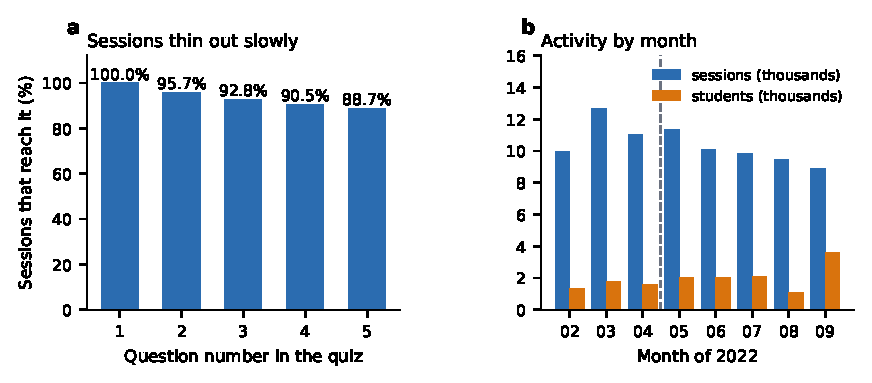
\includegraphics[width=0.95\textwidth]{../results/figures/fig2_overview.pdf}
\caption{The data. (a) Share of sessions that reach each question. (b) Sessions and students per month; the dashed line is the 3 May change found in Section~\ref{sec:q2}.}\label{fig:overview}\end{figure}

\subsection{How each question is answered}
\textbf{RQ1 (the lesson).} We take every failed retry that was followed by a check-out question (\qOneRoute{} cases, \qOneStudents{} students). The outcome is a correct first check-out answer. We split students into four groups by lesson time: skipped, glanced (10 s or less), read (up to 60 s) and long. Students who skip are not like the others, so we compare five estimates: the raw difference, the same students with and without a lesson, student fixed effects with controls, an adjusted logistic regression, and inverse-probability weighting. As a placebo test we ask if studying the lesson also predicts accuracy \emph{elsewhere} in the session, which should not happen if the lesson itself matters. We also report the E-value \citep{vanderweele2017evalue}, which says how strong a hidden confounder would need to be.

\textbf{RQ2 (where students quit).} We first compute the exit rate at each step type. Then we use a \emph{discrete-time hazard model} \citep{singer1993about}: every step is one row, and a logistic regression predicts ``did the session end here, given that it got here''. We add the ingredients one by one (event type, question number, failures so far, answer speed and time in session, calendar and year group) and compare them by 5-fold cross-validated AUC where the folds are made of whole students. For the failed-retry step we also fit a \emph{conditional logit with student fixed effects}, which compares a student only with themselves. This separates ``risk really changes'' from ``persistent students stay''. A likelihood-ratio scan finds a calendar break, and we repeat the main result with other exit definitions.

\textbf{RQ3 (persistence and return).} We order the sessions of each student. For persistence we compare the quit rate after a quit with the rate after a finished session, by the gap between the two sessions. To separate trait from state, we control for the student's own usual quit rate (leaving out the current session), fit a within-student model, and measure split-half reliability. For return we measure the time from the end of a session to the next session of the same student with Kaplan-Meier curves \citep{kaplan1958nonparametric}, where students who never come back before 30 September are treated as censored. We also fit a clustered logit for returning within 1 day and 7 days.

\subsection{Tools and statistics}
All code is in Python (pandas, NumPy, SciPy, statsmodels, scikit-learn, matplotlib) and the report is written in \LaTeX. Because the steps of one student are not independent, every interval is a 95\% interval from a student-cluster bootstrap (whole students resampled, seed 610) or from standard errors clustered by student. We report effect sizes with intervals, AUC and log-loss from cross-validation, standardised differences for balance, and permutation p-values for the ICCs. The code and one \texttt{run\_all} command that rebuilds every table, figure and number in this report are at \url{\repourl}.

\section{Results}
\subsection{RQ1: Is the lesson step linked to learning?}
Students who skipped the lesson got the check-out question right \qOneSuccSkip{} of the time (\qOneSuccSkipCI), students who only glanced \qOneSuccGlance, students who read it (median \qOneMedRead\,s) \qOneSuccRead{} and students who studied for long \qOneSuccLong{} (Figure~\ref{fig:q1}a). Success rises quickly until about 15 to 20 seconds and then stays flat. A glance does no better than a skip, so it seems the lesson has to be actually read.

The raw gap (\qOneEffRaw\pp, \qOneEffRawCI) is too big because skippers are different. They are in much worse sessions: \qOneSkipEarlierFail{} earlier failures on average against \qOneLessonEarlierFail{} for students who studied (standardised difference \qOneSMDfail; Figure~\ref{fig:q1}b). When we adjust, the effect shrinks to about half but stays clearly positive: \qOneEffFE\pp{} with student fixed effects (\qOneEffFECI), \qOneEffLogit\pp{} with the adjusted logit and \qOneEffIPW\pp{} with weighting (Figure~\ref{fig:q1}c; adjusted odds ratio \qOneOR, \qOneORCI). Inside the same student, compared with skipping, a glance adds only \qOneDoseFEGlance\pp{}, reading adds \qOneDoseFERead\pp{} and long study \qOneDoseFELong\pp. The result is similar before and after 3 May (\qOneFEBefore\pp{} and \qOneFEAfter\pp), without long gaps, and for questions 1 to 4 only. The placebo test is clean: studying the lesson does not predict accuracy elsewhere in the session once students are compared with themselves (\qOnePlacebo\pp, \qOnePlaceboCI), although the raw gap there is large (\qOnePlaceboRaw\pp). A hidden confounder would need to be linked to both lesson study and success with a risk ratio of about \qOneEvalue{} to remove the estimate (\qOneEvalueCI{} for the interval limit).

\begin{figure}[t]\centering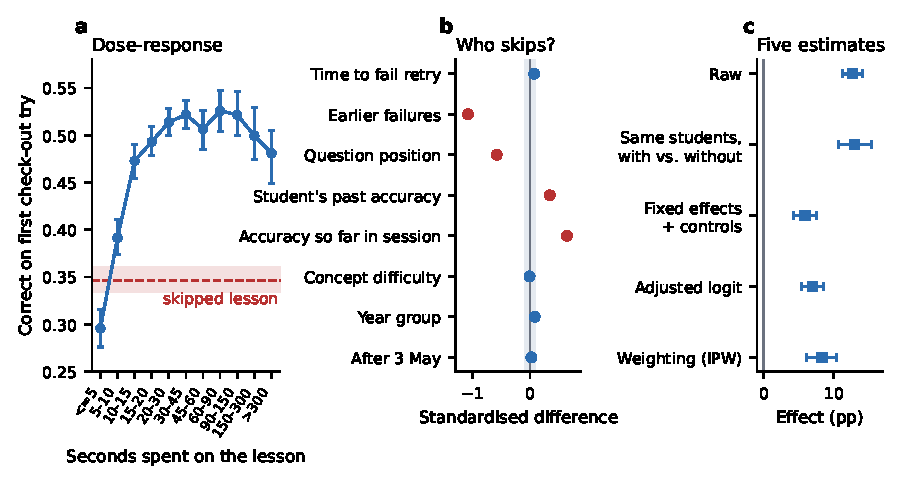
\includegraphics[width=\textwidth]{../results/figures/fig3_lesson.pdf}
\caption{RQ1. (a) First-try check-out success by lesson time; the band is the success of students who skipped. (b) How lesson and skip groups differ before adjustment (shaded: within $\pm0.1$). (c) Five estimates of the lesson effect, in percentage points with 95\% CI.}\label{fig:q1}\end{figure}

\subsection{RQ2: Where in a session does quitting concentrate?}\label{sec:q2}
\textbf{One step stands out.} A wrong check-in retry ends the session \qTwoRateFR{} of the time (\qTwoRateFRCI), against \qTwoRateOther{} at all other steps, a ratio of \qTwoRatio{} (\qTwoRatioCI). This one step makes \qTwoShareFR{} of all \nExits{} exits (Figure~\ref{fig:q2}a). If we average per student instead of per step the rate is \qTwoStudentRateFR{} (\qTwoStudentRateFRCI), so a few heavy users are not driving it. After such a failure \qTwoToLesson{} go to the lesson, \qTwoToCheckout{} go straight to the check-out and \qTwoToQuit{} quit. Once in the lesson students almost never quit (\qTwoQuitAfterLesson{}), and after a wrong check-out students who skipped the lesson quit \qTwoCommitNoLesson{} of the time against \qTwoCommitLesson{} for students who studied it. Part of this is the platform forcing a retry after a lesson, so we see the lesson as a point of no return, not as proof of motivation. The result is robust to the exit definition (Table~\ref{tab:sens}): the ratio stays between 10.6 and 15.6.

\begin{table}[t]\centering\small
\caption{The RQ2 headline with other exit definitions and samples.}\label{tab:sens}
\resizebox{\textwidth}{!}{\begin{tabular}{lrrrr}
\toprule
Exit definition / sample & Exits & After failed retry (\%) & Elsewhere (\%) & Ratio (95\% CI) \\
\midrule
Primary (session ended before Q5) & 9{,}426 & 13.1 & 0.94 & 13.9 (13.0 to 14.9) \\
+ any pause over 1 h counts as exit & 19{,}470 & 23.3 & 2.19 & 10.6 (10.1 to 11.2) \\
Exit and no return within 24 h & 5{,}930 & 7.4 & 0.67 & 11.0 (10.4 to 11.7) \\
Drop sessions in last 24 h of data & 9{,}419 & 13.1 & 0.94 & 13.9 (13.0 to 14.8) \\
Exclude first session of each student & 7{,}391 & 12.0 & 0.77 & 15.6 (14.4 to 16.9) \\
School-hours sessions only & 4{,}908 & 16.9 & 1.34 & 12.5 (11.7 to 13.3) \\
Years 5 to 11 only & 9{,}092 & 12.9 & 0.93 & 13.9 (13.0 to 15.0) \\
\bottomrule
\end{tabular}
}\end{table}

\textbf{Position, time and time of day.} At the failed-retry step the raw quit rate falls from \whereFROne{} at question 1 to \whereFRFour{} at question 4, and the rate at other steps also falls, from \whereOthOne{} to \whereOthFour{} (Figure~\ref{fig:where}a). Over the minutes of a session the quit rate after a failed retry falls from \whereTimeFirst{} in the first 30 seconds to about \whereTimeLast{} after 8 minutes. Quits at other steps follow a U-shape instead (\whereOthTimeMid{} at 1 to 2 minutes, \whereOthTimeLast{} after 8; Figure~\ref{fig:where}b). Quitting is highest during school hours and drops after school: after 3 May it is \whereHourPeak{} at 13 to 14 h against \whereHourDip{} at 15 to 16 h (Figure~\ref{fig:where}c).

\begin{figure}[t]\centering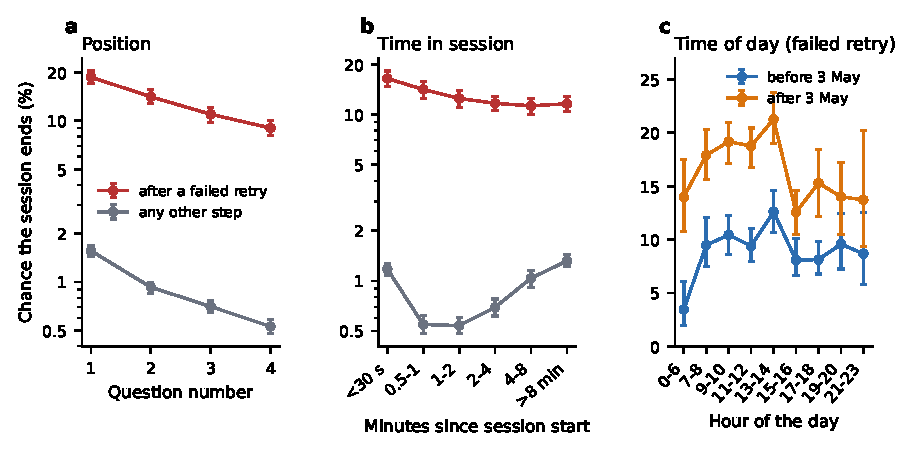
\includegraphics[width=\textwidth]{../results/figures/fig4_where.pdf}
\caption{RQ2. Chance a session ends (log scale in a and b; 95\% student-cluster CI). (a) By question number. (b) By time since the session started. (c) By hour of the day at failed-retry steps, before and after 3 May.}\label{fig:where}\end{figure}

\textbf{Which ingredients matter?} Every temporal ingredient helps predict exits of unseen students (Table~\ref{tab:hazard}): event type alone gives AUC \hzAUCA, question number \hzAUCB, answer speed and time in session \hzAUCD, and calendar and year group \hzAUCE. Failures so far add nothing once the question number is included (\hzAUCB{} vs.\ \hzAUCC). After a failed retry the adjusted quit chance is \hzMargPosOne{} at question 1 and \hzMargPosFour{} at question 4, and it is lower after very fast answers (\hzMargLatA{} within 3 s against \hzMargLatD{} at 12 to 25 s).

\begin{table}[t]\centering\small
\caption{Nested hazard models of quitting (5-fold CV, folds made of whole students).}\label{tab:hazard}
\resizebox{\textwidth}{!}{\begin{tabular}{lrrrr}
\toprule
Hazard model & Par. & McFadden $R^2$ & CV AUC & CV log-loss \\
\midrule
M0 event type & 8 & 0.161 & 0.769 & 0.0816 \\
M1 + position in quiz & 11 & 0.173 & 0.804 & 0.0804 \\
M2 + failures so far & 14 & 0.174 & 0.803 & 0.0803 \\
M3 + answering speed, time in session & 17 & 0.185 & 0.824 & 0.0792 \\
M4 + calendar and student context & 27 & 0.215 & 0.853 & 0.0766 \\
\bottomrule
\end{tabular}
}\end{table}

\textbf{Survivor effect.} In the pooled data more earlier failures seem to \emph{lower} the quit risk (adjusted \hzMargFailZero{} with none against \hzMargFailThree{} with three; odds ratio \hzPoolFailOne{} for one). The within-student model flips this: for the same student one earlier failed retry \emph{raises} the odds of quitting (OR \hzFEFailOne, \hzFEFailOneCI) and two raise them more (\hzFEFailTwo, \hzFEFailTwoCI; \hzFEstudents{} students who both quit and continued). The question-number effect stays (question 4 vs.\ 1: OR \hzFEPosFour) and the speed effect disappears (Figure~\ref{fig:q2}c). So the falling quit rate across a session is mostly persistent students staying, while each extra failure is risky for the individual.

\textbf{A change on 3 May.} The quit rate after a failed retry jumped from \cpBefore{} to \cpAfter{} on \cpDate{} 2022 (95\% interval \cpLo{} to \cpHi; likelihood-ratio statistic \cpLR; Figure~\ref{fig:q2}d). It shows up in the \cpPairN{} students seen in both periods (\cpPairDiff\pp, \cpPairCI) and in every year group. The quit rate at other steps also rose (\cpOtherBefore{} to \cpOtherAfter), so it is not only about failure. The documentation does not explain it, so we only control for it. The ratio between the failed-retry rate and the baseline hardly changes (\qTwoRatioBefore{} before, \qTwoRatioAfter{} after). Finally, students differ much more than topics: the student ICC is \qTwoICCStudent{} (\qTwoICCStudentCI), against \qTwoICCConcept{} for concepts and \qTwoICCTopic{} for subjects.

\begin{figure}[t]\centering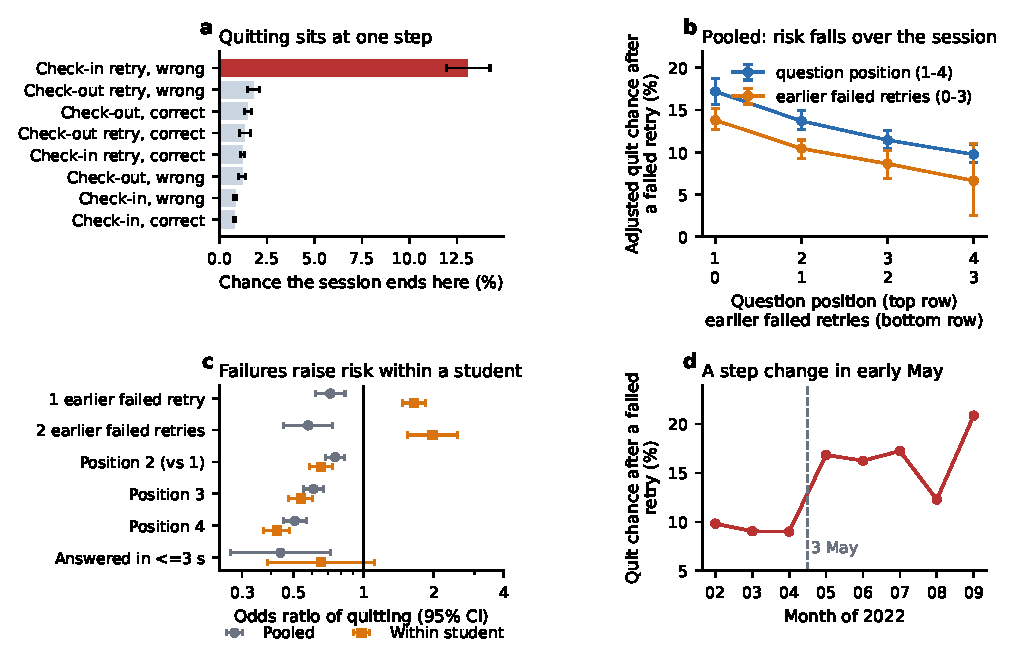
\includegraphics[width=0.97\textwidth]{../results/figures/fig5_quitting.pdf}
\caption{RQ2. (a) Chance a session ends at each step type. (b) Adjusted quit chance after a failed retry by question number and by earlier failures. (c) Odds ratios of quitting, pooled and within student. (d) Monthly quit chance after a failed retry; the dashed line is the detected change.}\label{fig:q2}\end{figure}

\subsection{RQ3: Is quitting persistent, and do quitters return?}
\textbf{Persistence.} After a quit the next session ends in a quit \qThreeAfterExit{} of the time, against \qThreeAfterComplete{} after a finished session (ratio \qThreeRatio, \qThreeRatioCI; \qThreePairs{} pairs of sessions). This holds for every gap, even for gaps over a week (ratio \qThreeWeek), so it is not just the same sitting continuing (\qThreeSame{} within an hour). A run of recent quits makes it stronger: the next session ends in a quit \streakZero{} of the time after 0 quits in the last 3 sessions, \streakOne{} after 1, \streakTwo{} after 2 and \streakThree{} after 3 (Figure~\ref{fig:q3b}c). Most of this is the student, not the last session. The extra risk after a quit goes from \qThreeRaw\pp{} (\qThreeRawCI) to \qThreeLoo\pp{} when we control for the student's usual quit rate, and to \qThreeWithin\pp{} (\qThreeWithinCI) when each student is compared only with themselves (Figure~\ref{fig:q3}c). Quitting is a stable habit: the split-half reliability is \qThreeSB{} (\qThreeSplitN{} students), \qThreeNever{} of students with 5 or more sessions never quit, and the top tenth make \qThreeTop{} of all quits (Gini coefficient \qThreeGini; Figure~\ref{fig:q3b}a and b).

\begin{figure}[t]\centering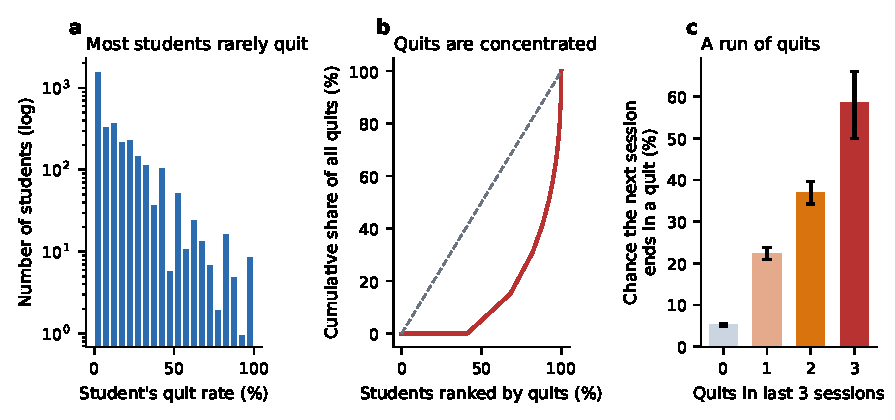
\includegraphics[width=\textwidth]{../results/figures/fig7_concentration.pdf}
\caption{RQ3. Students with 5 or more sessions. (a) Distribution of each student's quit rate. (b) Cumulative share of all quits when students are ranked from fewest to most quits (dashed: equal). (c) Chance the next session ends in a quit by number of quits in the last 3 sessions (95\% CI).}\label{fig:q3b}\end{figure}

\textbf{Return.} A quit is rarely final (Table~\ref{tab:return}, Figure~\ref{fig:q3}a), but quitters come back less than finishers. After a quit following a failed retry, \qThreeRetFRH{} start another session within an hour (median gap of those who return: \qThreeMedFR), \qThreeRetFRD{} within a day and \qThreeRetFRM{} within 30 days, against \qThreeRetDoneM{} after a finished session. Other quits are slower and less likely to be followed by a return (\qThreeRetOthD{} within a day, median \qThreeMedOth). After adjusting for period, weekend and experience, the odds of returning within a day are \qThreeORFRD{} (\qThreeORFRDCI) after a failed-retry quit and \qThreeOROthD{} after another quit, compared with finishing; within a week they are \qThreeORFRW{} and \qThreeOROthW. Almost nobody returns to the \emph{same} quiz (\qThreeSameQuizFR), so ``return'' means coming back to the platform.

\begin{table}[t]\centering\small
\caption{Share of students who start another session within the given time after a session ended (\%, 95\% CI; Kaplan-Meier, censored at the end of the data).}\label{tab:return}
\resizebox{\textwidth}{!}{\begin{tabular}{lrcccc}
\toprule
Previous session & $n$ & 1 h & 24 h & 7 d & 30 d \\
\midrule
Quit after failed retry & 5{,}328 & 37.6 (34.8 to 40.5) & 43.6 (40.4 to 46.6) & 56.5 (53.3 to 59.5) & 65.8 (63.2 to 68.2) \\
Other quit & 4{,}098 & 23.4 (21.3 to 25.3) & 28.7 (26.3 to 30.6) & 42.0 (39.2 to 44.4) & 52.1 (49.5 to 54.5) \\
Completed & 73{,}798 & 47.7 (45.7 to 50.0) & 63.6 (62.5 to 65.0) & 85.3 (84.5 to 85.9) & 90.4 (89.9 to 90.9) \\
\bottomrule
\end{tabular}
}\end{table}

\begin{figure}[t]\centering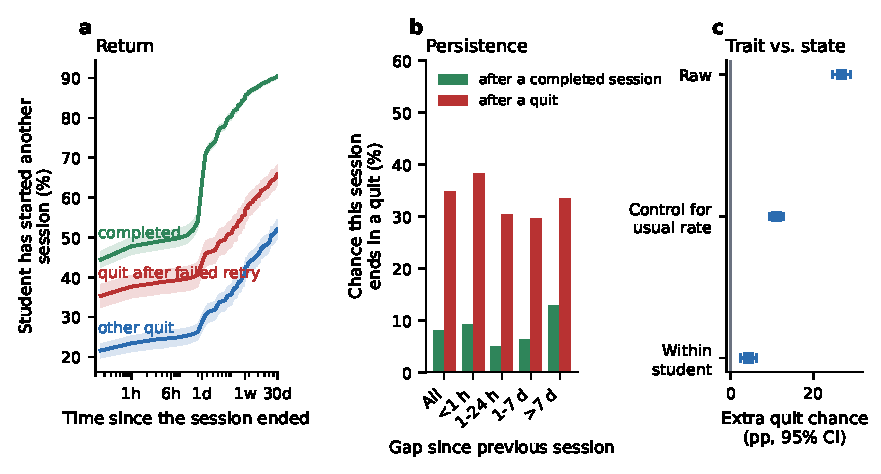
\includegraphics[width=\textwidth]{../results/figures/fig6_persistence_return.pdf}
\caption{RQ3. (a) Return curves with 95\% bands. (b) Chance a session ends in a quit by the previous session and the gap since it. (c) Extra quit chance after a quit under three models (pp = percentage points).}\label{fig:q3}\end{figure}

\section{Discussion and Limitations}
\subsection{What the results say about our hypotheses}
\begin{table}[t]\centering\small
\caption{Hypotheses and what we found.}\label{tab:verdict}
\begin{tabular}{@{}p{0.8cm}p{4.5cm}p{7.9cm}p{1.9cm}@{}}
\toprule
 & Hypothesis & Finding & Verdict\\\midrule
H1 & Lesson study goes with higher check-out success, more study helps up to a point & $+$\qOneEffRaw\pp{} raw, $+$\qOneEffFE\pp{} within student; flat after about 20 s; placebo clean & Supported\\
H2 & Quitting is concentrated after a failed retry and depends on position & \qTwoRatio$\times$ the rate at other steps; falls with position and time; but the pooled fall with failures is a survivor effect & Supported, with a twist\\
H3 & A quit predicts a quit, mostly via the student; quitters return less & $\times$\qThreeRatio{} pooled, $+$\qThreeWithin\pp{} within student; back within a week: \qThreeRetFRW{} vs.\ \qThreeRetDoneW & Supported\\
\bottomrule\end{tabular}\end{table}
The three results fit one story. A failed retry is the decision point. Most students go on to the lesson and the lesson is linked to a better next answer, but about one student in eight leaves at that moment, and those students come back less often. Quitting sits in one moment (after a failed retry), in the early part of a session and in a small group of students. The drop in quitting across a session mostly shows who is left, not that failure becomes easier. Looking at the same student, each extra failure makes stopping more likely.

\subsection{Practical meaning}
(i) A prompt that makes the lesson attractive right after a failed retry would target the biggest leak. (ii) Because quitting is a habit of some students, the few students with repeated quits are better targets for support than everyone. (iii) A quit followed by a return within minutes is probably an interruption, so dashboards should separate it from real drop-out. (iv) Changes like the one on 3 May should be checked before comparing months.

\subsection{Limitations}\label{sec:lim}
\begin{itemize}
\item \textbf{Observational data.} The lesson result is an association. Students choose to study, and the placebo test and E-value help but cannot prove a cause.
\item \textbf{No emotion measured.} We see exits, not frustration or boredom, so we only say ``quit after failed retry''.
\item \textbf{Platform rules.} The retry and lesson rules limit what students can do (for example a retry is forced after a lesson), so low quitting after a lesson is partly built in.
\item \textbf{Exit definition.} An exit can be an interruption. The ratio stays above 10 for all definitions we tried, but the absolute rates change a lot (\qTwoRateFR{} to 23.3\%).
\item \textbf{Return.} Return means any later session. It says nothing about learning, and \qThreeCensored{} of last sessions are censored at the end of the data.
\item \textbf{Unexplained break.} The 3 May change is controlled for but we do not know its cause.
\item \textbf{Data scope.} One platform, maths only, Years 5 to 11, and no class or teacher IDs, so students in the same class cannot be grouped. We could not model learning curves across sessions because most student-concept pairs appear only once.
\end{itemize}

\section{Conclusion}
We asked three questions about what happens when students fail in short Eedi quizzes, and each one gave a clear answer. For \textbf{RQ1}, the lesson step is linked to learning: students who read the lesson answered the check-out question about \qOneEffFE{} to \qOneEffIPW{} percentage points more often after we adjusted, and about half of the raw gap of \qOneEffRaw{} points was selection. The benefit needs real reading, since a glance is no better than a skip, and it levels off after about 20 seconds. For \textbf{RQ2}, quitting is not spread evenly. It piles up right after a wrong check-in retry, where the session ends \qTwoRateFR{} of the time, and it is stronger early in the quiz and in school hours. The finding we like most is the survivor effect: pooled data says failures make students more persistent, but the same students show the opposite, so a naive analysis would give the wrong lesson. For \textbf{RQ3}, quitting is persistent, but mostly because of who the student is. The extra risk from the last session is only \qThreeWithin{} points within a student, while a few students produce most quits. Quitters do come back, and quickly after a failed retry, but fewer return within a week than after a finished session.

For teachers and designers this suggests helping students at the moment of the first failed retry, for example by making the lesson feel useful and short, and keeping an eye on the small group of repeat quitters. For analysts it shows that quit and return data need within-student comparisons, a clear exit definition and a check for sudden calendar changes. There are limits (Section~\ref{sec:lim}): the data is observational, we do not see emotions and the 3 May change is unexplained. Next steps could be an experiment with a lesson prompt after the failed retry, linking the data to class and teacher information, and a model for return time that treats ``quit for good'' and ``come back later'' as competing outcomes. Doing this project also showed us how much careful definitions matter: the same data can tell a very different story depending on what we call a quit and who we compare with whom.

\begingroup\small
\begin{thebibliography}{9}
\bibitem[{Baker et~al.(2010)}]{baker2010frustrated} Baker, R. S. J. d., D'Mello, S. K., Rodrigo, M. M. T., \& Graesser, A. C. (2010). Better to be frustrated than bored: The incidence, persistence, and impact of learners' cognitive-affective states during interactions with three different computer-based learning environments. \emph{International Journal of Human-Computer Studies, 68}(4), 223-241. \url{https://doi.org/10.1016/j.ijhcs.2009.12.003}
\bibitem[{Beck \& Gong(2013)}]{beck2013wheel} Beck, J. E., \& Gong, Y. (2013). Wheel-spinning: Students who fail to master a skill. In \emph{Artificial Intelligence in Education} (pp. 431-440). Springer. \url{https://doi.org/10.1007/978-3-642-39112-5_44}
\bibitem[{Gong et~al.(2022)}]{gong2022causal} Gong, W., Smith, D., Wang, Z., Barton, C., Woodhead, S., Pawlowski, N., Jennings, J., \& Zhang, C. (2022). \emph{NeurIPS competition instructions and guide: Causal insights for learning paths in education} (arXiv:2208.12610). \url{https://arxiv.org/abs/2208.12610}
\bibitem[{Kaplan \& Meier(1958)}]{kaplan1958nonparametric} Kaplan, E. L., \& Meier, P. (1958). Nonparametric estimation from incomplete observations. \emph{Journal of the American Statistical Association, 53}(282), 457-481. \url{https://doi.org/10.1080/01621459.1958.10501452}
\bibitem[{Singer \& Willett(1993)}]{singer1993about} Singer, J. D., \& Willett, J. B. (1993). It's about time: Using discrete-time survival analysis to study duration and the timing of events. \emph{Journal of Educational Statistics, 18}(2), 155-195. \url{https://doi.org/10.3102/10769986018002155}
\bibitem[{VanderWeele \& Ding(2017)}]{vanderweele2017evalue} VanderWeele, T. J., \& Ding, P. (2017). Sensitivity analysis in observational research: Introducing the E-value. \emph{Annals of Internal Medicine, 167}(4), 268-274. \url{https://doi.org/10.7326/M16-2607}
\end{thebibliography}
\endgroup
\end{document}
